% ============================================================
% Figure 1: YOLOv14 System Pipeline (CVPR single-column)
% Compile with: pdflatex -> xelatex + shell-escape
% ============================================================
\documentclass[tikz,border=5pt]{standalone}
\usepackage{tikz}
\usetikzlibrary{shapes,arrows,positioning,fit,backgrounds,calc}
\usepackage{amsmath,amssymb}

\tikzset{
  block/.style={rectangle, rounded corners=4pt, draw, minimum width=2.8cm,
                minimum height=1.0cm, text centered, font=\small\bfseries, fill=#1!15,
                draw=#1!60, thick},
  data/.style={trapezium, trapezium left angle=70, trapezium right angle=110,
               draw, minimum width=2.2cm, minimum height=0.9cm,
               text centered, font=\small, fill=orange!15, draw=orange!60, thick},
  arrow/.style={->, >=stealth, thick},
  darrow/.style={->, >=stealth, thick, dashed, gray},
  loss/.style={rectangle, draw, minimum width=2.2cm, minimum height=0.7cm,
               fill=red!10, draw=red!60, thick, font=\small},
  box/.style={rectangle, draw, dashed, inner sep=5pt, rounded corners=2pt,
              label={[font=\small\itshape]above:#1}},
}

\begin{document}
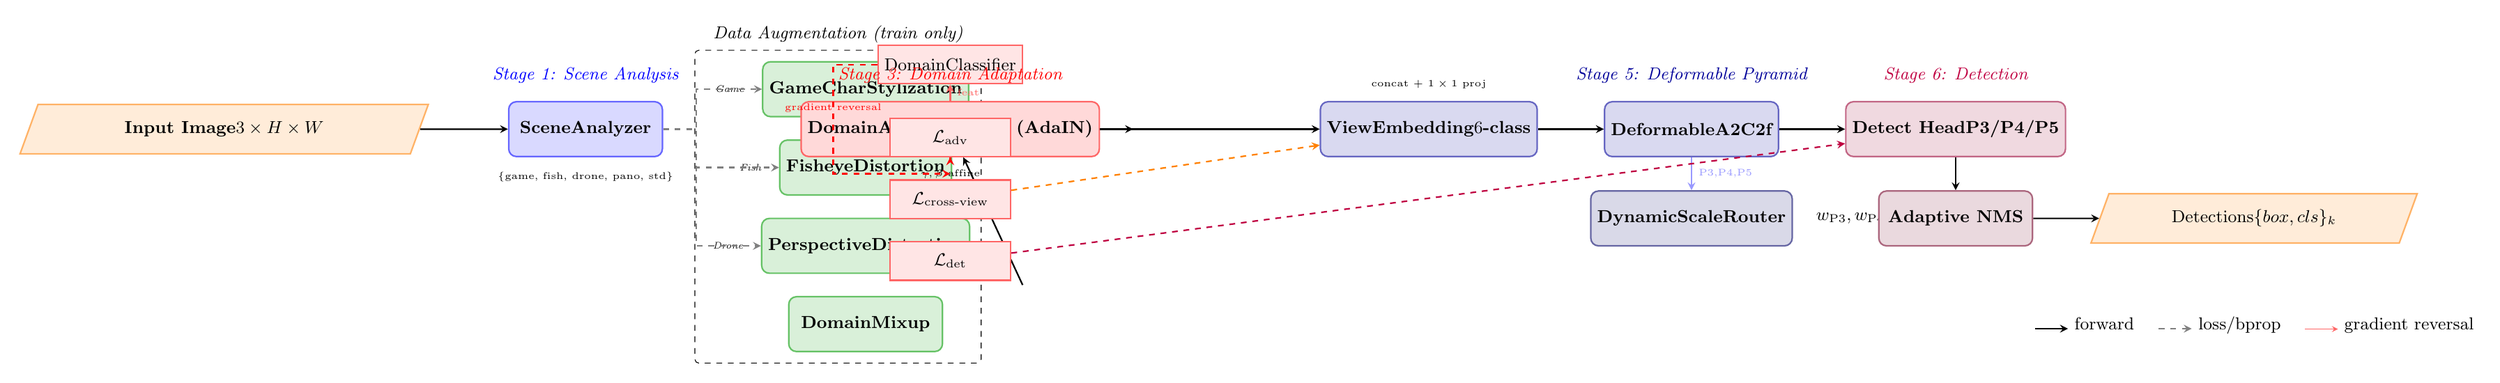
\begin{tikzpicture}[node distance=1.0cm and 1.2cm]

% -------------------- Input --------------------
\node[data] (input) {\textbf{Input Image}\\$3\times H\times W$};

% -------------------- Stage 1: Scene Analysis --------------------
\node[block={blue}, right=1.6cm of input] (scene) {Scene\\Analyzer};
\node[below=0.15cm of scene, font=\tiny] (scenes) {\{game, fish, drone, pano, std\}};

\draw[arrow] (input) -- (scene);

% -------------------- Stage 2: Adaptive Augmentation (dashed box) --------------------
\begin{scope}[local bounding box=augbox]
  \node[block={green!60!black}, above right=-0.3cm and 1.8cm of scene] (game)
      {GameChar\\Stylization};
  \node[block={green!60!black}, below=0.4cm of game] (fisheye)
      {Fisheye\\Distortion};
  \node[block={green!60!black}, below=0.4cm of fisheye] (persp)
      {Perspective\\Distortion};
  \node[block={green!60!black}, below=0.4cm of persp] (mixup)
      {Domain\\Mixup};
  \node[left=0.2cm of game, font=\tiny\itshape] {Game};
  \node[left=0.2cm of fisheye, font=\tiny\itshape] {Fish};
  \node[left=0.2cm of persp, font=\tiny\itshape] {Drone};
\end{scope}
\node[fit={(augbox)}, box={Data Augmentation (train only)}, inner sep=6pt] {};
\draw[darrow] (scene.east) -- ++(0.6,0) |- (game.west);
\draw[darrow] (scene.east) -- ++(0.6,0) |- (fisheye.west);
\draw[darrow] (scene.east) -- ++(0.6,0) |- (persp.west);

\coordinate (augout) at ($(mixup.east)!0.5!(persp.east) + (1.2,0)$);

% -------------------- Stage 3: Domain Adaptation --------------------
\node[block={red}, right=2.5cm of scene] (domain)
    {DomainAdaptive\\Layer (AdaIN)};
\node[below=0.1cm of domain, font=\tiny] {$\gamma,\beta$ affine};
\draw[arrow] (domain.east) -- ++(0.6,0);
\draw[arrow] (augout) -- (domain);

\coordinate[right=0.6cm of domain] (mid);

% -------------------- Classifier + adversarial loss --------------------
\node[loss, above=0.3cm of domain] (cls) {Domain\\Classifier};
\draw[->, >=stealth, thick, red!60] (domain.north) -- (cls.south)
    node[midway, right, font=\tiny] {feat};
\draw[darrow, red] (cls.west) -- ++(-0.8,0) |- ($(domain.south)+(0,-0.3)$)
    node[pos=0.25, above, font=\tiny, red] {gradient reversal};

% -------------------- Stage 4: View Conditioning --------------------
\node[block={blue!60!black}, right=4.0cm of domain] (view)
    {ViewEmbedding\\$6$-class};
\node[above=0.1cm of view, font=\tiny] {concat + $1\times1$ proj};
\draw[arrow] (domain.east) -- (view);

% -------------------- Stage 5: Deformable Pyramid --------------------
\node[block={blue!60!black}, right=of view] (deform)
    {DeformableA2C2f};
\draw[arrow] (view.east) -- (deform);

\node[block={blue!40!black}, below=0.6cm of deform] (router)
    {DynamicScale\\Router};
\draw[->, >=stealth, thick, blue!40] (deform.south) -- (router.north)
    node[midway, right, font=\tiny] {P3,P4,P5};

\node[right=0.3cm of router, font=\small] {$w_{\text{P3}},w_{\text{P4}},w_{\text{P5}}$};

% -------------------- Stage 6: Detection --------------------
\node[block={purple!80!black}, right=of deform] (detect)
    {Detect Head\\P3/P4/P5};
\draw[arrow] (deform.east) -- (detect);

\node[block={purple!60!black}, below=0.6cm of detect] (nms)
    {Adaptive NMS};
\draw[arrow] (detect.south) -- (nms.north);

\node[data, right=of nms] (output) {Detections\\$\{box, cls\}_{k}$};
\draw[arrow] (nms.east) -- (output);

% -------------------- Losses --------------------
\node[loss, below=0.6cm of cls] (advloss) {$\mathcal{L}_{\text{adv}}$};
\node[loss, below=0.4cm of advloss] (cvloss) {$\mathcal{L}_{\text{cross-view}}$};
\node[loss, below=0.4cm of cvloss] (detloss) {$\mathcal{L}_{\text{det}}$};

\draw[darrow, red] (advloss) -- (domain);
\draw[darrow, orange] (cvloss) -- (view);
\draw[darrow, purple] (detloss) -- (detect);

% -------------------- Labels --------------------
\node[above=0.2cm of scene, font=\small\itshape, blue] {Stage 1: Scene Analysis};
\node[above=0.2cm of domain, font=\small\itshape, red] {Stage 3: Domain Adaptation};
\node[above=0.2cm of deform, font=\small\itshape, blue!60!black] {Stage 5: Deformable Pyramid};
\node[above=0.2cm of detect, font=\small\itshape, purple] {Stage 6: Detection};

% legend
\node[below=1.2cm of output, font=\small] (legend) {
  \tikz\draw[arrow] (0,0) -- (0.6,0); forward \quad
  \tikz\draw[darrow] (0,0) -- (0.6,0); loss/bprop \quad
  \tikz\draw[->, >=stealth, red!60] (0,0) -- (0.6,0); gradient reversal
};

\end{tikzpicture}
\end{document}
